\section{Определение языка}

Вдохновением данной работы послужила статьи~\cite{Palmgren} и~\cite{isaev}. Поэтому сам язык спецификации выглядит как язык описания алгебраических теорий.

Начнем с примера языка с зависимыми типами~(рис.\ref{lpi})~\cite[Глава~2.1]{book:pierce}

\begin{figure}
    \centering
	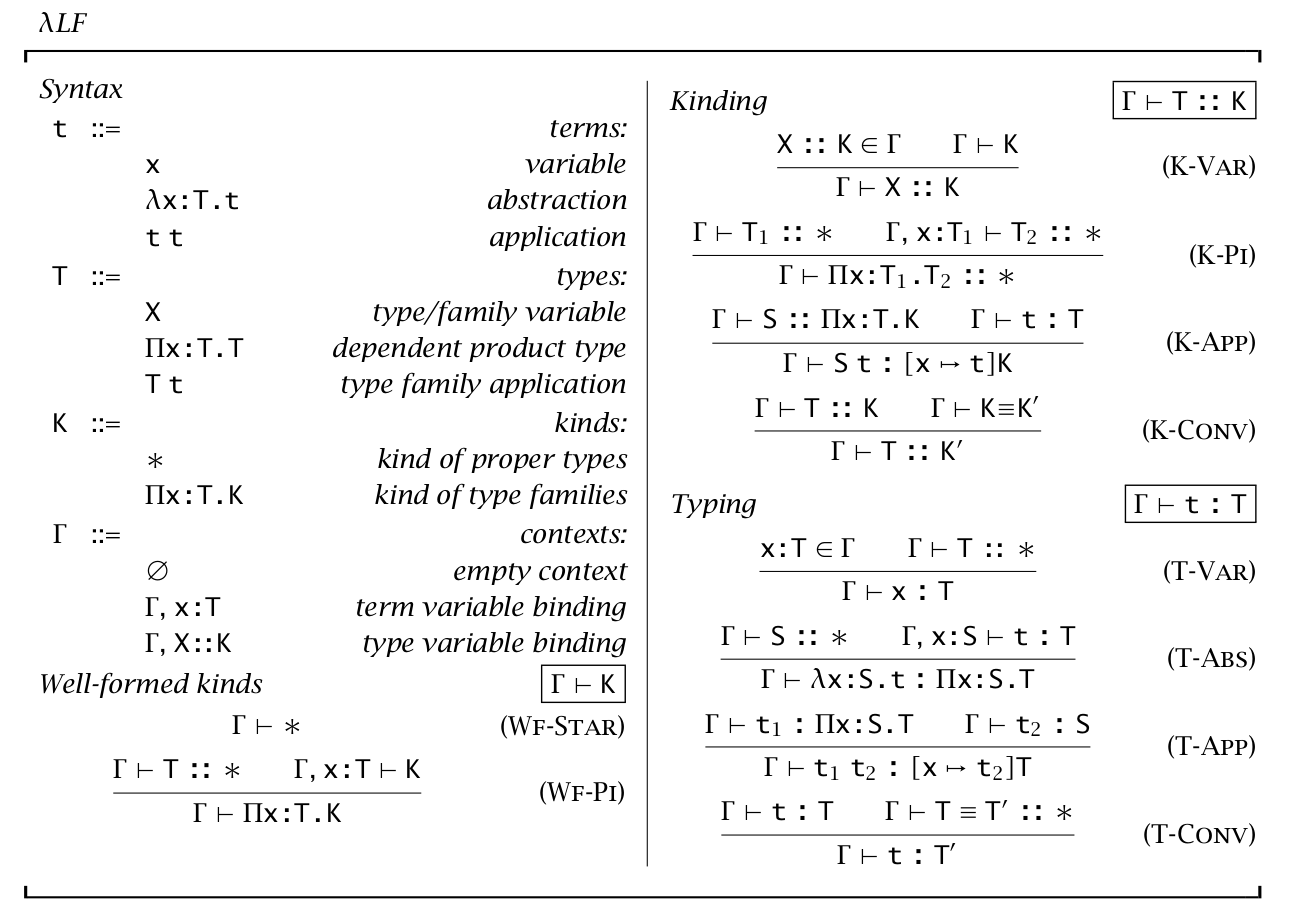
\includegraphics[scale=0.35]{img/lp.png}
	\caption{Язык с лямбдой и $\Pi$-типами }
	\label{lpi}
\end{figure}

Так этот язык будет выглядеть в нашем языке\footnote{правила связанные с кайндами опущены для простоты}

\begin{lstlisting}
DependentSorts:
  tm, ty
FunctionalSymbols:
  lam: (ty, 0)*(tm, 1) -> tm
  app: (tm, 0)*(tm, 0)*(ty, 1) -> tm
  pi : (ty, 0)*(ty, 1) -> ty
Axioms:
  K-Pi =
    forall T1 : ty, x.T2 : ty
      x : T1 |- T2 def |--- |- pi(T1, x.T2) def

  TAbs =
    forall S : ty, x.T : ty, x.t : tm
      x : S |- t : T |--- |- lam(S, x.t) : pi(S, x.T)
  TApp =
    forall t1 : tm, t2 : tm, S : ty, x.T : ty
            |- t1 : pi(S, x.T),
            |- t2 : S,
      x : S |- T def
      |--------------------------
      |- app(t1, t2, x.T) : T[x:=t2]
Reductions:
  Beta =
    forall x.b : tm, A : ty, a : tm, z.T : ty
       |--- |- app(lam(A, x.b), a, z.T) => b[x:=a] : T[z:=a]

\end{lstlisting}

\subsection{Ограничения на спецификации, налагаемые языком}

\begin{enumerate}

\item Все используемые метапеременные должны иметь аннотацию (сорт), то есть присутствовать в секции forall аксиомы/редукции.

\item Запрещено равенство в заключении аксиом, для определенности каждого шага в проверке типов определяемого языка (если видим равенство не ясно в какую сторону идти при редуцировании)

\item Все аргументы в функциональный символ в заключении аксиомы должны быть метапеременными. Ещё и с теми же аргуементами что и в forall (не больше).

\item Если в заключении аксиомы написан функциональный символ возвращающий сорт, он обязан также иметь тип (нельзя просто написать $ \vdash f(\ldots) def$).

\item Определения функциональных символов всегда одно, иначе появляется недетерминированность в проверке типов. Не играет особой роли, тк в данном случае можно сделать недетерминированность в проверке.

\item Подстановки разрешены только в метапеременные - в принципе это слабое ограничение, которое облегчает жизнь при реализации, не ограничивая пользователя.

\item В заключении контекст не должен быть расширен - это ограничение связано с тем, что иначе смысл аксиомы становится странным. А именно: функциональный символ применим только при введении перепенных в контекст.

\item \label{tm:Meta} Все метапеременные используемые в предпосылках должны либо присутствовать в метапеременных заключения или же должны быть типами какой-либо предпосылки.

\item Если в функциональном символе встречаются метапеременные с контекстами $x_1 \ldots x_k . T$, должна существовать предпосылка вида $x_1 : S_1 \ldots x_k : S_k  \vdash T$. Это сделано для того чтобы не передавать типы контекстов метапеременных функционального символа явно.

\item Если метапеременная является типом предпосылки и не встречается в аргументах функционального символа, то она может использоваться только справа от двоеточия. Таким образом избегаются ситуации связанные с порядком проверки предпосылок языка. А именно: если у нас есть $x : S \vdash t : T, x:T \vdash r : S$. То нужно строить граф зависимостей для предпосылок и использовать порядок полученный в результате его топологической сортировки в генерации кода. (Аналогично с~\ref{toposort}).

\item Все переменные контекстов метапеременных могут использовать только метапеременные левее внутри функционального символа в заключении - это связано с тем, что иначе могут возникнуть циклы в определениях метапеременных: S тип с аргументом типа R, R тип с аргументом типа S, S тип с аргументом типа R...

\item Из-за ослабления условия на метапеременные в пункте~\ref{tm:Meta}, порядок метапеременных неочевиден. Решение данной проблемы описано в секции~\ref{toposort}.

\item Редукции не учитывают предпосылок при приведении в нормальную форму - предполагается что они не конфликтуют с аксиомами и проверки в аксиомах достаточно.

\item В редукциях все метапеременные справа от '=>' должны встречаться и слева от него.

\item Подстановка запрещена слева от '=>'.



\end{enumerate}

\subsection{Проверки корректности спецификации языка}

Тривиальными проверками, осуществляемыми после парсинга языка, являются: проверка того, что сорты используемых выражений совпадают с аргументами функциональных символов.
